
%(BEGIN_QUESTION)
% Copyright 2009, Tony R. Kuphaldt, released under the Creative Commons Attribution License (v 1.0)
% This means you may do almost anything with this work of mine, so long as you give me proper credit

Examine this P\&ID for a cascaded gas-pressure control system:

$$\includegraphics[width=15.5cm]{i00079x01.eps}$$

Assuming both transmitters are direct-indicating (i.e. greater pressure/flow results in greater signal to the respective controllers), determine the necessary control actions (direct or reverse) for each controller.  In addition to determining ``direct'' or ``reverse'' action for each controller, label each controller's inputs with ``+'' and ``$-$'' symbols showing the direction of action for PV and for SP individually.

\vskip 10pt

\begin{itemize}
\item{} Pressure Indicating Controller (PIC): {\it direct} or {\it reverse} action?
\vskip 10pt 
\item{} Flow Indicating Controller (FIC): {\it direct} or {\it reverse} action?
\end{itemize}

\vskip 20pt \vbox{\hrule \hbox{\strut \vrule{} {\bf Suggestions for Socratic discussion} \vrule} \hrule}

\begin{itemize}
\item{} What must be configured in the FIC to allow the operator to see 0-100\% (registered on the controller faceplate) as true valve position (i.e. 0\% on faceplate = shut valve and 100\% on faceplate = open valve)?
\item{} Would your answer(s) be different if the control valve throttled gas {\it leaving} the vessel rather than gas {\it entering} the vessel?  This, of course, would mean that at least one of the (currently) out-going pipes would have to supply gas to the vessel instead.
\item{} Would your answer(s) be different if the control valve were fail-closed (FC) instead of fail-open (FO)?
\item{} Would your answer(s) be different if the flow transmitter were located downstream of the control valve instead of upstream?
\item{} Describe the purpose of the device labeled ``PSV'' in this diagram.
\end{itemize}

\underbar{file i00079}
%(END_QUESTION)





%(BEGIN_ANSWER)

To aid your analysis of the system (especially in labeling each controller's inputs with ``+'' and ``$-$'' symbols), feel free to annotate the controller actions in this modified version of the P\&ID, where each controller is drawn as an operational amplifier:

$$\includegraphics[width=15.5cm]{i00079x02.eps}$$

%(END_ANSWER)





%(BEGIN_NOTES)

$$\includegraphics[width=15.5cm]{i00079x03.eps}$$










\filbreak \vskip 20pt \vbox{\hrule \hbox{\strut \vrule{} {\bf Virtual Troubleshooting} \vrule} \hrule}

\noindent
{\bf Predicting the effect of a given fault:} present each of the following faults to the students, one at a time, having them comment on all the effects each fault would produce.

\begin{itemize}
\item{} 
\item{} 
\item{} 
\end{itemize}


\vskip 10pt


\noindent
{\bf Identifying possible/impossible faults:} present symptoms to the students and then have them determine whether or not a series of suggested faults could account for all the symptoms, explaining {\it why} or {\it why not} for each proposed fault:

\begin{itemize}
\item{} Symptom: {\it }
\item{}  -- {\bf Yes/No}
\item{}  -- {\bf Yes/No}
\item{}  -- {\bf Yes/No}
\end{itemize}


\vskip 10pt


\noindent
{\bf Determining the utility of given diagnostic tests:} present symptoms to the students and then propose the following diagnostic tests one by one.  Students rate the value of each test, determining whether or not it would give useful information (i.e. tell us something we don't already know).  Students determine what different results for each test would indicate about the fault, if anything:

\begin{itemize}
\item{} Symptom: {\it Pressure in gas accumulator vessel is oscillating around setpoint}
\item{} Put the PIC into manual mode -- {\bf Yes}
\item{} Check calibration of PT -- {\bf No}
\item{} Check calibration of FT -- {\bf No}
\item{} Put the FIC into manual mode -- {\bf Yes}
\item{} Examine phase shift between PV and SP of PIC -- {\bf No}
\item{} Examine phase shift between PV and Output of PIC -- {\bf Yes}
\item{} Decrease gain of PIC -- {\bf Yes}
\item{} Monitor gas demand flows (if FTs exist downstream) -- {\bf Yes}
\end{itemize}


\vskip 10pt


\noindent
{\bf Diagnosing a fault based on given symptoms:} imagine the ??? fails ??? in this system (don't reveal the fault to students!).  Present the operator's observation(s) to the students, have them consider possible faults and diagnostic strategies, and then tell them the results of tests they propose based on the following symptoms, until they have properly identified the nature and location of the fault:

\begin{itemize}
\item{} Operator observation: {\it }
\item{} 
\item{} 
\end{itemize}

















\vfil \eject

\noindent
{\bf Summary Quiz:}

Identify the effect of the flow transmitter failing with a {\it high} signal (i.e. reporting full flow all the time) on this cascaded gas pressure control system:

$$\includegraphics[width=15.5cm]{i00079x01.eps}$$

\begin{itemize}
\item{} The control valve will fail wide open
\vskip 5pt 
\item{} The accumulator gas pressure will fall below setpoint
\vskip 5pt 
\item{} Flow through the ``Gas Demand'' lines will greatly increase
\vskip 5pt 
\item{} The accumulator gas pressure will rise above setpoint 
\vskip 5pt 
\item{} The flow controller will begin to ``cycle'' (oscillate)
\vskip 5pt 
\item{} There will be no effect(s) whatsoever on the control system
\end{itemize}

%INDEX% Control, strategies: cascaded controller action
%INDEX% Process: fuel gas receiver pressure control

%(END_NOTES)


